\begin{apendicesenv}

\chapter{Projeto do \textit{Data Warehouse}}

\section{Modelo Dimensional do \textit{Data Warehouse}}

O modelo dimensional do \textit{data warehouse} foi modelado utilizado a ferramenta MySQL Workbench ~\footnote{MySQL Workbench Community possui licença GPL 2.0 e pode ser encontrado em \url{http://dev.mysql.com/downloads/tools/workbench/}} e pode ser visto na Figura \ref{esquema}.

\begin{figure}[ht!]
\centering
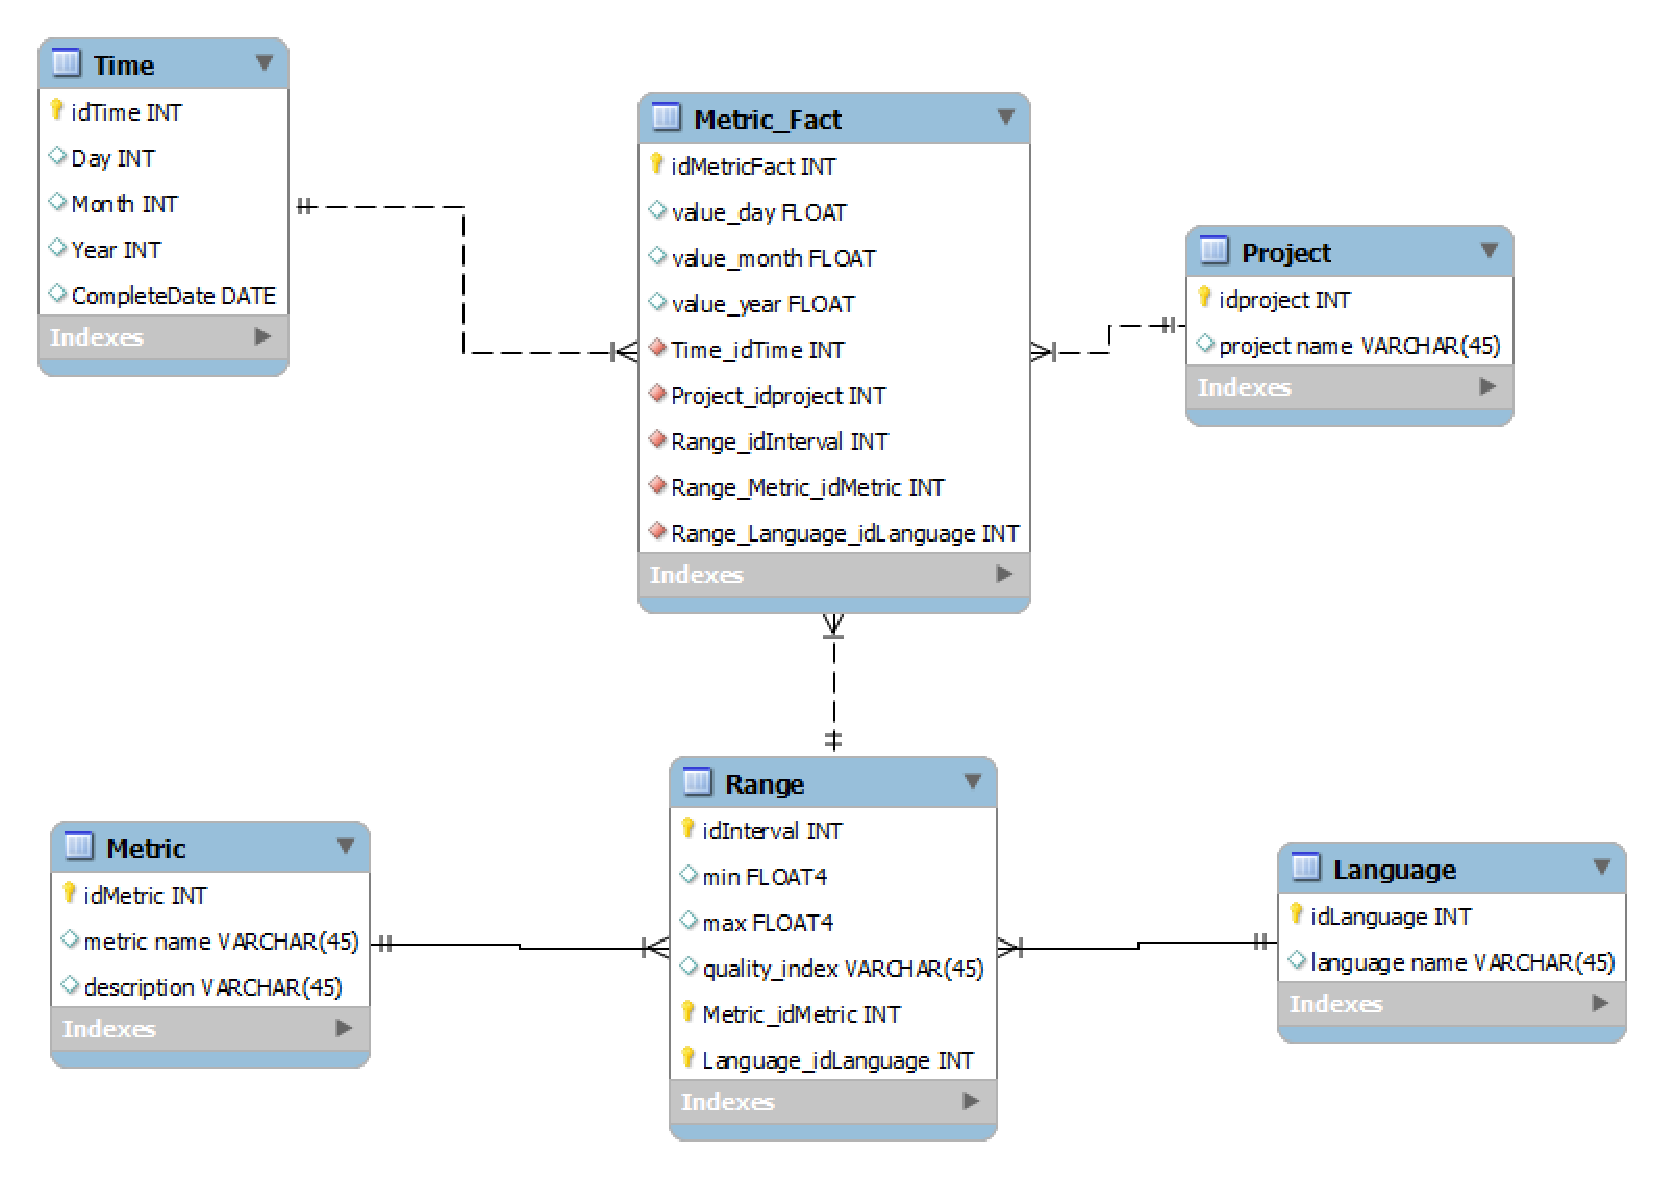
\includegraphics[keepaspectratio=false,scale=0.60]{apendices/esquema.eps}
\caption{Modelo Dimensional do \textit{Data Warehouse}}
\label{esquema}
\end{figure}
\FloatBarrier

\clearpage
\section{SQL do Data Warehouse}
\label{sql-datawarehouse}
\lstset{
		 language = SQL,	
         basicstyle=\footnotesize\ttfamily, % Standardschrift
         numbers=left,               % Ort der Zeilennummern
         numberstyle=\tiny,          % Stil der Zeilennummern
         %stepnumber=2,               % Abstand zwischen den Zeilennummern
         numbersep=5pt,              % Abstand der Nummern zum Text
         tabsize=1,                  % Groesse von Tabs
         extendedchars=true,         %
         breaklines=false,            % Zeilen werden Umgebrochen
         keywordstyle=\color{blue},
    		frame=b,         
 %        keywordstyle=[1]\textbf,    % Stil der Keywords
 %        keywordstyle=[2]\textbf,    %
 %        keywordstyle=[3]\textbf,    %
 %        keywordstyle=[4]\textbf,   \sqrt{\sqrt{}} %
  		 identifierstyle=\color{BrickRed},
         stringstyle=\color{OliveGreen}\ttfamily,
         commentstyle=\color{Sepia}, % Farbe der String
         showspaces=false,           % Leerzeichen anzeigen ?
         showtabs=false,             % Tabs anzeigen ?
         xleftmargin=\parindent,
         framexleftmargin=17pt,
         framexrightmargin=5pt,
         framexbottommargin=4pt,
         %backgroundcolor=\color{lightgray},
         showstringspaces=false      % Leerzeichen in Strings anzeigen ?        
 }
\lstinputlisting{apendices/schema.sql}


%\chapter{Segundo Apêndice}
%
%Texto do segundo apêndice.

\end{apendicesenv}
